\documentclass{beamer}

\usepackage[utf8]{inputenc}
\usepackage{default}
\usepackage{listings}

\usetheme[alternativetitlepage=true,% Use the fancy title page.
          titlepagelogo=roadrunner-book.png]{Torino}

\begin{document}

\title{Is That Book Checked Out?}
\subtitle{Getting Holdings and Availability Data into Other Applications}
\author{Jane Sandberg}
\institute{Linn-Benton Community College}

\renewcommand{\figurename}{Credit}

\begin{frame}
 \titlepage
\end{frame}


\begin{frame}{Background}
 \begin{itemize}
  \item Creating a new Discovery Layer
  \item Using Blacklight, because it's cool!
  \item Wanted real-time holdings data, but did not want to query the db directly.
 \end{itemize}

\end{frame}

\begin{frame}{I had already met SuperCat}

\begin{columns}

 \column{0.5\textwidth}
 \begin{figure}
  \begin{center}
   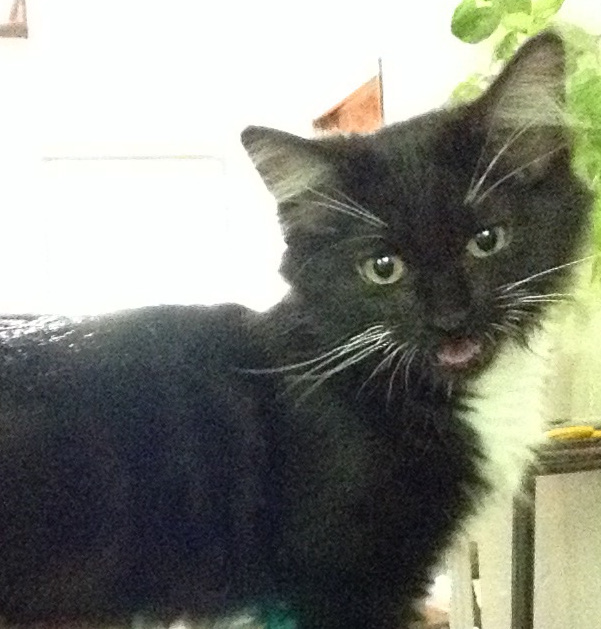
\includegraphics[height=2in]{supercat.jpg}
  \end{center}

 \end{figure}

  \column{0.4\textwidth}
\begin{itemize}
 \item Our consortium's sysadmin pointed me toward some documentation on the wiki
 \item I used it to create a cute display of our new books
\end{itemize}

\end{columns}
 
\end{frame}




\begin{frame}{SuperCat is nice!}

\begin{columns}

 \column{0.5\textwidth}
 \begin{figure}
  \begin{center}
   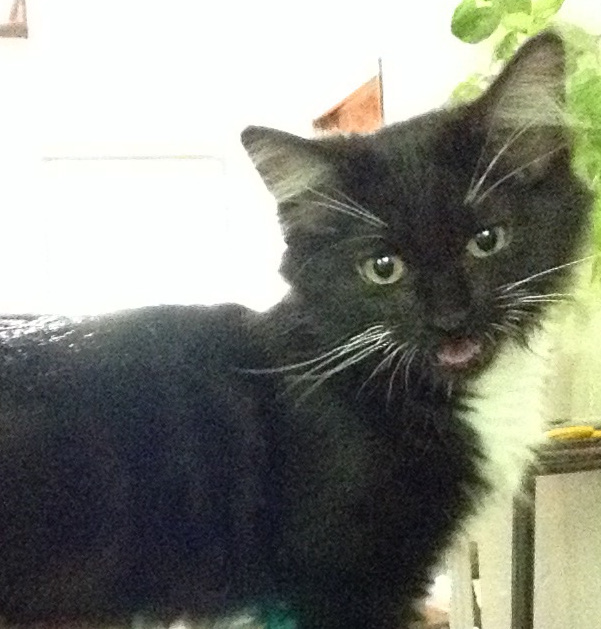
\includegraphics[height=2in]{supercat.jpg}
  \end{center}

 \end{figure}

  \column{0.4\textwidth}

\begin{block}<2->{Format was nice!}
I could easily parse the XML with nokogiri's xpath powers -- Blacklight already had this as a dependency!
\end{block}
\begin{block}<3->{Credentials required}
None!
\end{block}
\begin{block}<4->{Capabilities are clear}
Easy to get to list of possible formats. 
\end{block}
\end{columns}
 
\end{frame}

\begin{frame}{How to use SuperCat}

\begin{block}<1->{Format}

http://example.com/opac/extras/supercat/

\{COMMAND\}/

\{FORMAT\}/

\{Specific information needed by your COMMAND\}

\end{block}
\begin{block}<2->{Example SuperCat query}
 http://libcat.linnbenton.edu/opac/extras/supercat/retrieve/atom-full/record/514477
 
\end{block}
\end{frame}



\begin{frame}[fragile]{Results of Supercat query}

\begin{lstlisting}
[snip]

<counts>
  <count type="public" count="1" available="1" unshadow="1" transcendant="0" org_unit="1" depth="0"/>
  <count type="staff" count="1" available="1" unshadow="1" transcendant="0" org_unit="1" depth="0"/>
</counts>
<volumes>
  <volume id="tag:open-ils.org:asset-call_number/643383" lib="LBCCLIB" opac_visible="t" deleted="f" label="PN6733.T35 S87 2015">
    <copies>
      <copy id="tag:open-ils.org:asset-copy/442300" create_date="2016-02-29T16:39:58-0800" edit_date="2016-03-15T12:55:44-0700" copy_number="" circulate="t" deposit="f" ref="f" holdable="t" deleted="f" deposit_amount="0.00" price="" barcode="38813001196056" circ_modifier="DEFAULT" circ_as_type="" opac_visible="t">
        <status ident="0" opac_visible="t">Available</status>
        <location ident="223" opac_visible="t">New books</location>
        <circlib ident="7" opac_visible="t">LBCC Library</circlib>
[snip]
\end{lstlisting}
 
\end{frame}




\begin{frame}{Supercat isn't perfect}
 \begin{itemize}
  \item The atom-full format had everything I needed, but it also returns a bunch of other (bibliographic) data that we don't really need.
  \item htmlholdings-full format didn't have any helpful markup.  Also wasn't totally interested in dropping results in as an HTML list.
  \item Staff suggestion: display due datetime when item checked out
 \end{itemize}

\end{frame}


\begin{frame}{OpenSearch}

\begin{columns}

 \column{0.5\textwidth}
 \begin{figure}
  \begin{center}
   
\includegraphics[height=1in]{opensearch.jpg}
   \caption{Alan David Robb / CC0}
  \end{center}

 \end{figure}

  \column{0.4\textwidth}

\begin{block}<2->{Format was also nice!}
In fact, it had the same format options as supercat...
\end{block}
\begin{block}<3->{Credentials required}
None!
\end{block}
\begin{block}<4->{Capabilities are clear}
Because they are the same as supercat...
\end{block}
\end{columns}


 
\end{frame}


\begin{frame}{UnAPI}
 
 \begin{columns}
 \column{0.5\textwidth}
 \begin{figure}
  \begin{center}
   
\includegraphics[height=2in]{unapi.png}
   \caption{Public Domain Image}
  \end{center}

 \end{figure}


  \column{0.4\textwidth}

\begin{block}<2->{Format was almost ideal!}
holdings\_xml-full!
\end{block}
\begin{block}<3->{Credentials required}
None!
\end{block}
\begin{block}<4->{Capabilities are not clear}
Unless you read through Open-ILS/src/perlmods
/lib/OpenILS/WWW
/SuperCat.pm
\end{block}
\end{columns}
 
 
\end{frame}


\begin{frame}{UnAPI}
\begin{itemize}
 \item  URLs look like this:
 https://libcat.linnbenton.edu/opac/extras/unapi?
 id=tag:U2@bre:biblio\_record\_entry/280157\&
 format=holdings\_xml-full
\item Still don't have due dates in there.
\end{itemize}

 
 
\end{frame}




\begin{frame}{JSON from opensrf web gateway}
 
 \begin{columns}
 \column{0.5\textwidth}
 \begin{figure}
  \begin{center}
   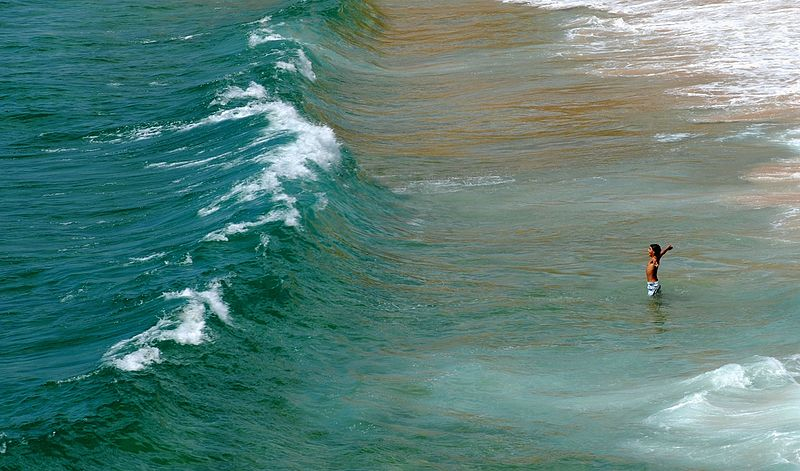
\includegraphics[height=1in]{opensrf.jpg}
   \caption{Joaquim Alves Gaspar / CC-BY-SA-3.0}
  \end{center}

 \end{figure}


  \column{0.4\textwidth}

\begin{block}<2->{Format is kinda scary}
But very compact!
\end{block}
\begin{block}<3->{Credentials required}
Authentication token
\end{block}
\begin{block}<4->{Capabilities are pretty much unlimited}
As long as Evergreen can do it, I can do it too.
\end{block}
\end{columns}


\end{frame}

\begin{frame}{JSON from opensrf web gateway}
 
 http://libcat.linnbenton.edu/gateway?
 
 service=open-ils.cat\&
 
 method=open-ils.cat.asset.copy\_tree.retrieve\&
 
 param=[AUTH TOKEN]\&
 
 param=294385\&param=7
 
\end{frame}

\renewcommand{\figurename}{How to get here}

\begin{frame}{Getting an auth token}
 \begin{figure}
  \begin{center}
   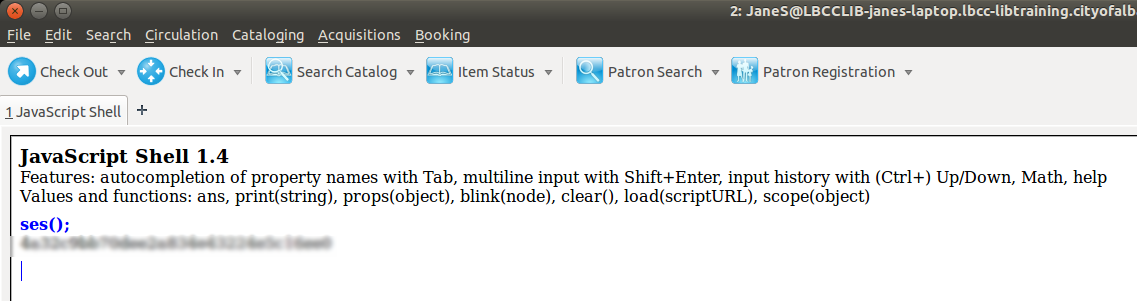
\includegraphics[height=1.7in]{ses.png}
   \caption{Admin $\rightarrow$ For developers $\rightarrow$ Javascript Shell}
  \end{center}

 \end{figure}


 
\end{frame}


\begin{frame}[fragile]{Results of opensrf query}

\begin{lstlisting}
{"payload":[[/*--S acn--*/[[],"2012-11-13T15:50:08
-0800",756052,"f","2012-11-13T15:50:08-0800",
756052,275533,"M1507.O5555 2003bx",7,294385,null,
null,null,"M1507 O5555  02003BX",/*--S acnc--*/[3,
"Library of Congress (LC)","asset.
label_normalizer_lc", "050ab,055ab,090abef"]
/*--E acnc--*/,/*--S acnp--*/[-1,"","",1]
/*--E acnp--*/,/*--S acns--*/[-1,"","",1]
/*--E acns--*/]/*--E acn--*/,/*--S acn--*/[[
/*--S acp--*/[null,null,"38813001133703",358160
,null,7,"DEFAULT","t",null,
"2012-11-13T15:51:31-0800",

[snip]

\end{lstlisting}
 
\end{frame}



\end{document}
